\chapter{Study Area}
Ob River (\autoref{fig:Ob Basin}), river of central Russia. One of the greatest rivers of Asia, the Ob flows north and west across western Siberia in a twisting diagonal from its sources in the Altai Mountains to its outlet through the Gulf of Ob into the Kara Sea of the Arctic Ocean. It is a major transportation artery, crossing territory at the heart of Russia that is extraordinarily varied in its physical environment and population. Even allowing for the barrenness of much of the region surrounding the lower course of the river and the ice-clogged waters into which it discharges, the Ob drains a region of great economic potential.\\\\
\begin{figure}[htbp]
	\centering
	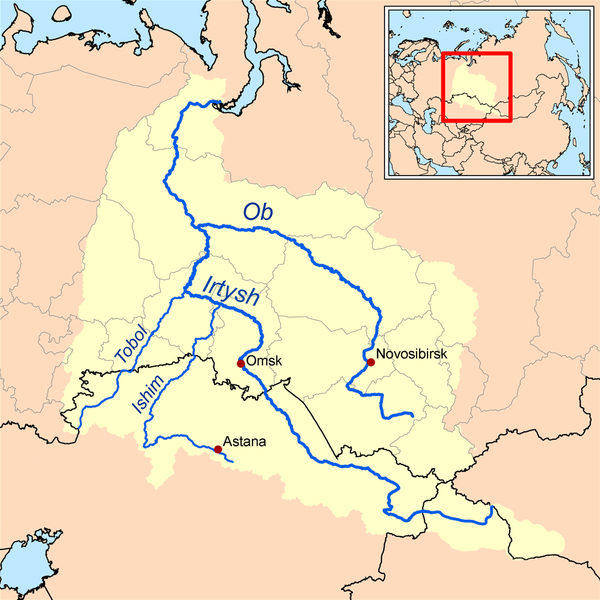
\includegraphics[width=0.7\textwidth]{Obbasin_area} % Datei in "bilder/" bei LaTeX: eps, bei PDFLaTeX: jpg (o.ä.) 
	\caption{River Basins Ob http://www.geologypage.com/2014/03/ob-river.html} 
	\label{fig:Ob Basin}
\end{figure}
\section{Physiography}
The Ob proper is formed by the junction of the Biya and Katun rivers, in the foothills of the Siberian sector of the Altai, from which it has a course of 3 650 km. If, however, the Irtysh River is regarded as part of the main course rather than as the Ob's major tributary, the maximum length, from the source of the Black (Chorny) Irtysh in China's sector of the Altai, is 5 410 km, making the Ob the seventh longest river in the world. The catchment area is approximately 2 975 000 square km. Constituting about half of the drainage basin of the Kara Sea, the Ob's catchment area is the sixth largest in the world. The drainage basin is classified as cropland (36\%), forest (30\%), wetland (11\%), grassland (10\%), shrub (5\%) , developed (5\%) and irrigated cropland (3\%).\cite{revenga1998watersheds}\\\\
The West Siberian Plain covers about 85 percent of the Ob basin.\cite{Obriver} The rest of the basin comprises the terraced plains of Turgay (Kazakhstan) and the small hills of northernmost Kazakhstan in the south and the Kuznetsk Alatau range, the Salair Ridge, the Altai Mountains and their foothills and outliers in the southeast.\\\\
The huge basin of the Ob stretches across a number of natural zones. Semidesert prevails in the far south around Lake Zaysan (recipient of the Black Irtysh and source of the Irtysh proper), bordered on the north by steppe grassland. The central regions of the West Siberian Plain i.e., more than half of the basin-consist of taiga (swampy coniferous forest), with great expanses of marshland. In the north there are vast stretches of tundra (low-lying, cold-tolerant vegetation).
\section{Climate}
According to Koeppen-Gerger climate classification, major part of Ob basin belongs to Subarctic climate(Dfc) \ref{fig:climate} \cite{peel2007updated}. It has short, warm summers and long, cold winters. Average January temperatures range from  $-28 ^{\circ}$C on the shores of the Kara Sea to $-16 ^{\circ}$C in the upper reaches of the Irtysh. July temperatures for the same locations, respectively, range from 4 $^{\circ}$C to above $20 ^{\circ}$C. The absolute maximum temperature, in the arid south, is $40 ^{\circ}$C,\cite{Obriver} and the minimum, in the Altai Mountains, is $-60 ^{\circ}$. Rainfall, which occurs mainly in the summer, averages less than 400 mm per year in the north, 500 to 600 mm in the taiga zone, and 300 to 400 mm on the steppes. The western slopes of the Altai receive as much as 1 575 mm per year. Snow cover lasts for 240 to 270 days in the north and for 160 to 170 days in the south. It is deepest in the forest zone, where it ranges from 60 to 90 cm, and in the mountains, where it averages 200 cm per year. It is much shallower on the tundra, ranging from 30 to 50 cm, and very thin on the steppe, where 20 to 40 cm fall.\cite{Obriver}\\\\
On the upper Ob the spring floods begin early in April, when the snow on the plains is melting; and they have a second phase, ensuing from the melting of snow on the Altai Mountains. The middle Ob, scarcely affected by the upper Ob's phases, has one continuous spring-summer period of high water, which begins in mid April. For the lower Ob, high water begins in late April or early May. Levels, in fact, begin to rise when the watercourse is still obstructed by ice; and maximum levels, which occur by May on the upper Ob, may not be reached until June, July, or even August on the lower reaches. For the upper Ob, the spring floods end by July, but autumn rains bring high water again in September and October; in the middle and lower Ob, the spring and summer floodwaters gradually recede until freezing sets in. On the lower reaches, flooding may last four months. Flooding of the Ob proper and of the Irtysh obstructs the minor tributaries' drainage.
\begin{figure}[htbp]
	\centering
	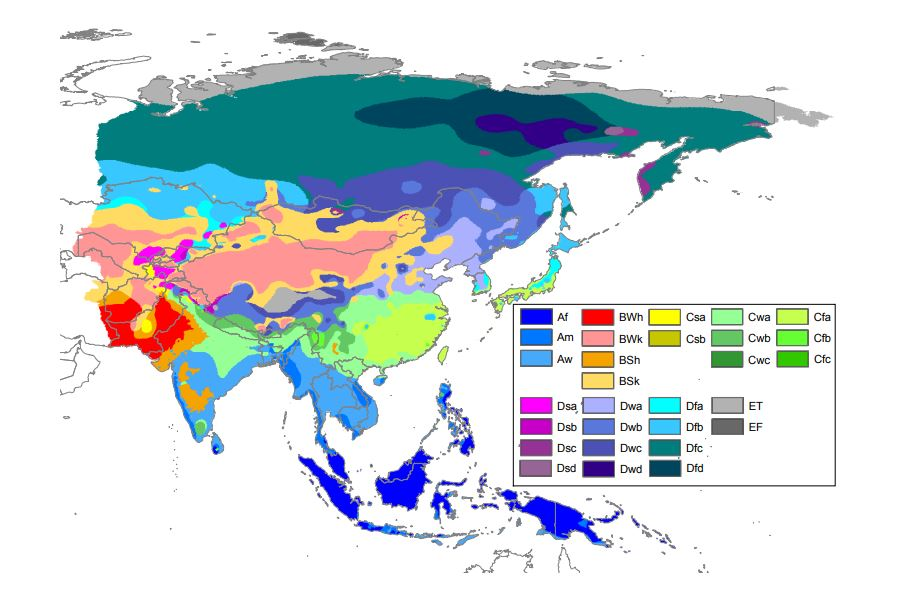
\includegraphics[width=0.8\textwidth]{climate} % Datei in "bilder/" bei LaTeX: eps, bei PDFLaTeX: jpg (o.ä.) 
	\caption{Asia Map of Koeppen-Geiger climate classification \cite{peel2007updated}} 
	\label{fig:climate}
\end{figure}
\section{Hydrology}
The Ob has the third greatest discharge of Siberia's rivers, after the Yenisey and the Lena. On average, it pours some 400 cubic km of water annually into the Arctic Ocean about 12\% of that ocean's total intake from drainage.
The volume of flow at Salekhard, just above the delta, is about 42 000 cubic metres per second at its maximum and 2 000 cubic metres per second at its minimum, while for Barnaul, on the upper Ob, the corresponding figures are 9 600 and 200 cubic metres per second. The average annual discharge rate at the river's mouth is about 12 700 cubic metres per second. Most of the water comes from the melting of seasonal snow and from rainfall; much less of it comes from groundwater, mountain snow, and glaciers.\cite{Obriver}
\section{Permafrost}
Permafrost is ground that continuously remains frozen for two or more years, located on land or under the ocean. Permafrost currently underlies significant portions of the six largest Arctic basin \cite{frey2009impacts} which include Ob river Basin. Permafrost is formed from ice holding various types of soil, sand, and rock in combination \cite{permafrost}. In recent years, as Earth's warms, the permafrost is thawing, which means the permafrost melts, leaving hebind water and soil \cite{permafrost}.
\section{Human use}
Basin total population is about 27 million, with 39 cities having a population of more than 100 000. The Ob's immense hydroelectric potential is estimated at some 250 billion kilowatts. Three main stations have been built: one on the Ob proper, at Novosibirsk, and the other two on the mountainous reaches of the Irtysh, at Bukhtarma and Oeskemen. Both industry and agriculture have been intensively developed in the Ob basin. Cities such as Omsk, Novosibirsk, and Barnaul are major industrial and manufacturing centres. The steppe zone, in the southern Ob basin, is the major producer of spring wheat in Russia. The west Siberian oil and gas fields, located in the taiga and tundra zones of the middle and lower Ob, are the most important in Russia, contributing about two-thirds of the country's crude oil and natural gas output.